\chapter{Guided auto-install}
\label{chapter:auto-install}

\section{Introduction}
Download the latest regadb-install.exe installation executable from the RegaDB website. Doubleclick the executable and the installer startup screen will appear.

\section{Stepping through the automatic installer}
\subsection{Acknowledge the license}
This page asks you to read the RegaDB license, which is the GNU Public License (GPLv2). Briefly, this license
provides you the right to use the software in any way you like, and
grants you the right to access and modify the underlying source code.

You may distribute the software further, provided that you keep the
license intact, and that you also give access to the source code (in
case made modifications).

You should be aware that the software comes with no warranty. 
\\
\vspace{0.5cm}~ \\ \centerline{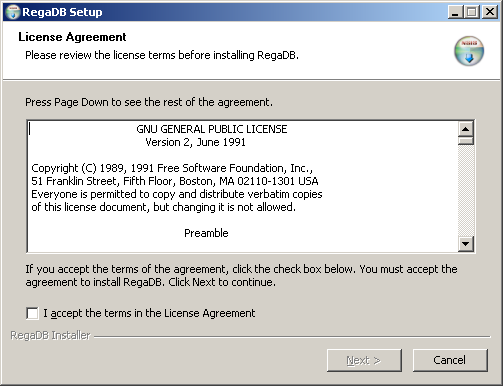
\includegraphics[width=8cm] {pics/nsis/license_agreement_1.png}}
\\
If you agree with the license enable the checbox and click \textbf{Next}.
\vspace{0.5cm}~ \\ \centerline{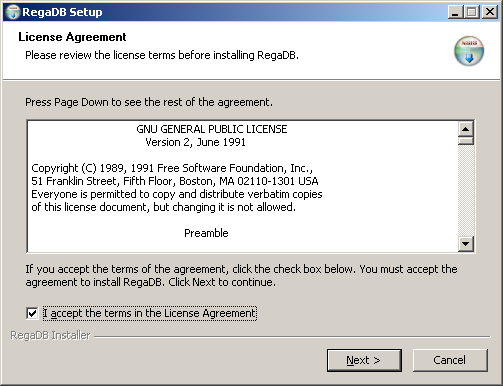
\includegraphics[width=8cm] {pics/nsis/license_agreement_2.png}}

\subsection{Select components to install}
Select all the modules for a completely automatic installation (default). Click \textbf{Next}.
\\\textit{If you only install the core module, some manual steps will be necessary after the guided installation procedure.}
\\
\vspace{0.5cm}~ \\ \centerline{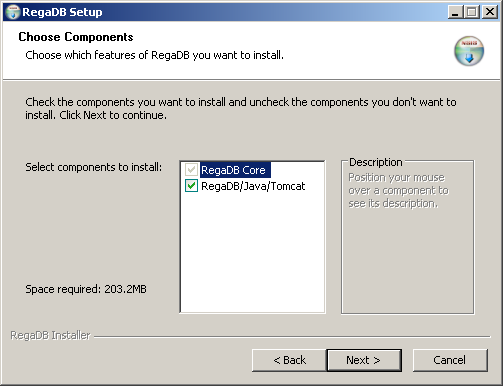
\includegraphics[width=8cm] {pics/nsis/select_components_3.png}}

\subsection{Specify the installation path}
The default installation path is preselected, if you agree with this installation path, please click \textbf{Next}.
\\
\vspace{0.5cm}~ \\ \centerline{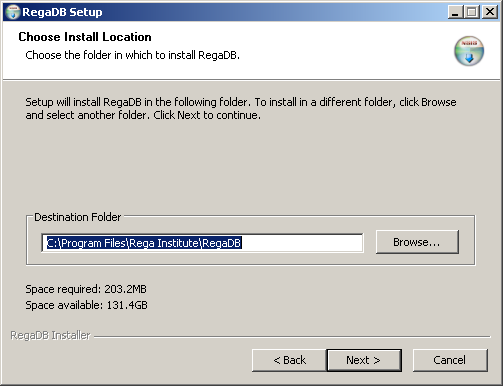
\includegraphics[width=8cm] {pics/nsis/installation_path_4.png}}
If you wish to have another installation path, click \textbf{Browse...} and select the appropriate installation directory.
\\
\vspace{0.5cm}~ \\ \centerline{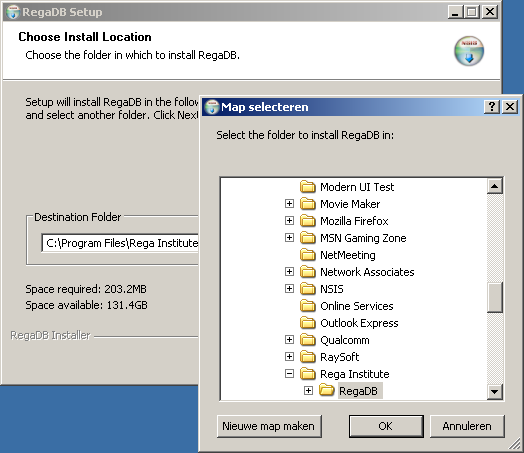
\includegraphics[width=8cm] {pics/nsis/installation_path_5.png}}


\subsection{Select the RDBMS to be used by RegaDB}
Please select the default database, this will enable RegaDB to use the Java RDBMS Hsqldb, than click \textbf{Next}.
\\
\vspace{0.5cm}~ \\ \centerline{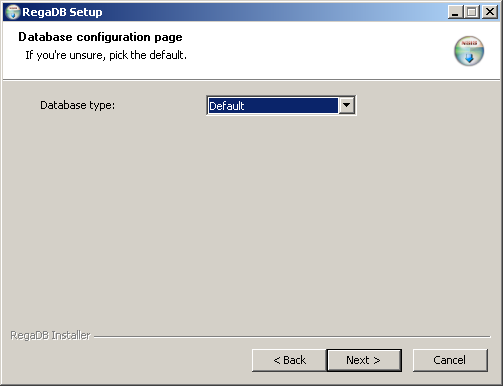
\includegraphics[width=8cm] {pics/nsis/select_database_6.png}}
\textit{If you select Postgresql in this page, further manual steps will be necessary.}

\subsection{Provide http proxy information}
While using RegaDB, the software requires internet access. Therefore, if your internet connection requires the use of a proxy, fill in your proxy settings. If you have a direct internet connection you may skip this step.
\\
\vspace{0.5cm}~ \\ \centerline{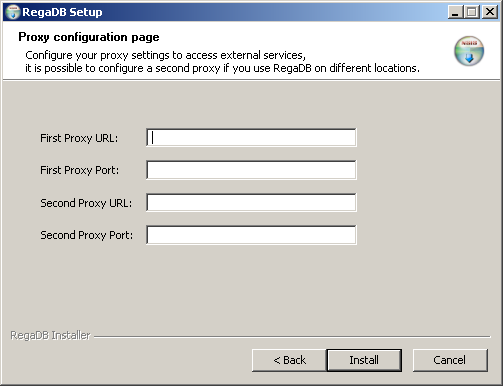
\includegraphics[width=8cm] {pics/nsis/select_proxy_7.png}}
Fill in your settings, and click \textbf{Next}. 
\\
\vspace{0.5cm}~ \\ \centerline{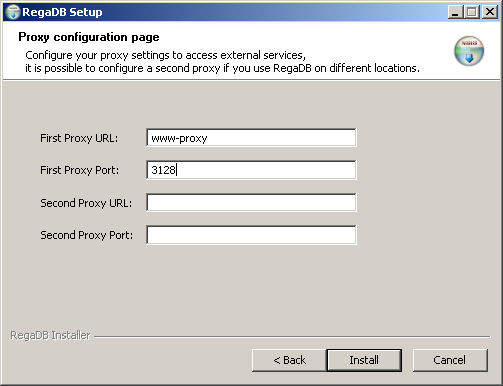
\includegraphics[width=8cm] {pics/nsis/select_proxy_8.png}}
RegaDB supports multiple proxy settings, and allows you to select the appropriate settings when you log in to the system.

\subsection{Installing the software}
Once all the configuration steps have been done, the software will be installed.
\\
\vspace{0.5cm}~ \\ \centerline{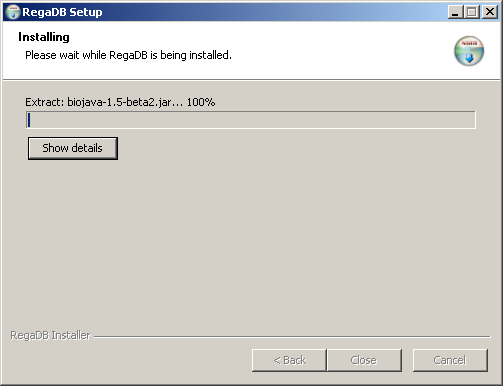
\includegraphics[width=8cm] {pics/nsis/installing_9.png}}
When the installation is complete, click \textbf{Close}. 
\\
\vspace{0.5cm}~ \\ \centerline{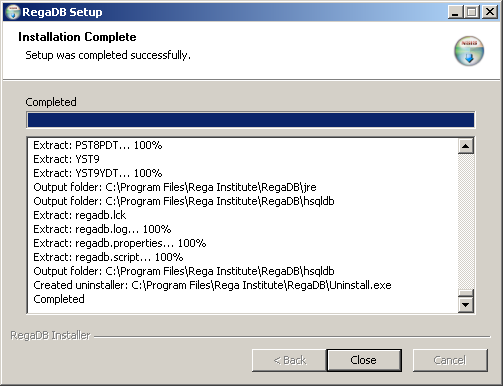
\includegraphics[width=8cm] {pics/nsis/installing_10.png}}
\\Please proceed to the Post installation chapter to finish the configuration of RegaDB (chapter~\ref{chapter:post_install}).
